\subsection{Machine Learning und Deep Learning}
\label{sec:MachineDeepLearning}

Machine Learning ist ein Teilgebiet der Informatik, das sich fundamental von der klassischen Programmierung unterscheidet.
Diese Unterscheidung wird von Chollet in \cite{DeepLearningPythonKeras} auf den Seiten 23 und 24 beschrieben.
In \autoref{fig:KlassischVsML} wird der Unterschied verdeutlicht.

\begin{figure}[h]
    \centering
    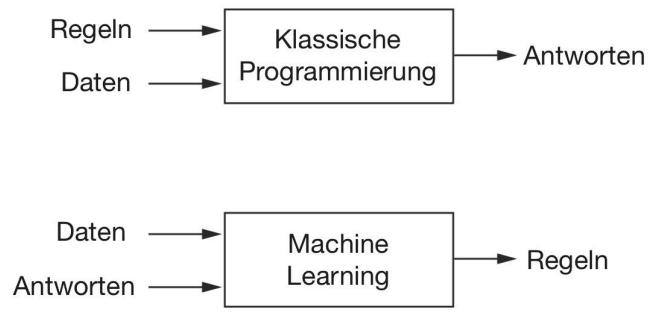
\includegraphics[width=0.5\textwidth,height=6cm,keepaspectratio=true]{content/images/KlassischVsML.png}
    \caption{Unterschied zwischen klassischer Programmierung und Machine Learning \cite[Abb.~1.2]{DeepLearningPythonKeras}}
    \label{fig:KlassischVsML}
\end{figure}

Sowohl klassische Programmierung als auch Machine Learning sollen im Rahmen von künstlicher Intelligenz verschiedenste Fragestellungen beantworten, die ansonsten von Menschen beantwortet werden.
Ein Beispiel für eine solche Fragestellung könnte z.\,B. lauten: "`Welche Ziffer ist in diesem Bild dargestellt?"'.
Ein anderes Beispiel wäre "`Gegeben ist dieser halbe Satz, wie könnte er weiter gehen?"'.
Die Fragestellung der vorliegenden Arbeit wurde bereits definiert.
Sie kann wie folgt in einem Satz zusammengefasst werden:
"`Gegeben sind die Standorte von mobilen Radarkontrollen der letzten 16 Tage, wie groß ist die Gefahr für mobile Radarkontrollen am 17. Tag an verschiedenen Stellen?"'
Bei der klassischen Programmierung liegt es nach Chollet nun am Menschen, Regeln aufzustellen, nach denen die Fragestellungen beantwortet werden.
Der Mensch könnte sich vergangene Daten anschauen und müsste in ihnen Muster suchen, von denen diese Regeln abgeleitet werden können.
Die Regeln werden anschließend in einer Programmiersprache explizit in Form von Verzweigungen, Schleifen und Variablen implementiert.
Für die Vorhersage von mobilen Radarkontrollen könnte ein Mensch beispielsweise aus eigener Erfahrung im Straßenverkehr gewisse Muster erkennen.
Daraus könnte z.\,B. die Regel aufgestellt werden, dass die Wahrscheinlichkeit für eine mobile Radarkontrolle an einem Standort sehr gering ist, wenn dort am vorherigen Tag bereits eine solche aufgestellt war.
Wie in \autoref{fig:KlassischVsML} zusammengefasst wird, findet die klassische Programmierung auf Basis von Eingangsdaten und explizit implementierten Regeln Antworten.

Beim Machine Learning ist es anders herum.
Ein Machine Learning Algorithmus erhält nach Chollet als Eingabe Daten und Antworten und leitet daraus Regeln ab.
Diese Regeln können anschließend verwendet werden, um anhand von neuen Eingabedaten neue Antworten zu erzeugen.
Die Regeln müssen nun also nicht mehr explizit vom Menschen festgelegt werden.
Dies bringt den Vorteil mit sich, dass möglicherweise Regeln erkannt werden, die dem Menschen (z.\,B. aufgrund ihrer Komplexität) verborgen blieben.
Für die Vorhersage von mobilen Radarkontrollen würde ein Machine Learning Algorithmus sehr viele Beispiele von je 16 aufeinanderfolgenden Tagen als Eingangsdaten sowie den 17. Tag als Antwort erhalten.
Anhand der daraus erlernten Regeln und 16 neuen Tagen als Eingabe, könnte dann der 17. Tag vorhergesagt werden.
Chollet beschreibt auf Seite 152, dass hierfür jedoch zwei Voraussetzungen erfüllt sein müssen:
Zum einen muss der 17. Tag anhand der 16 vorangegangenen Tage vorhersagbar sein.
Es muss also einen Zusammenhang zwischen Vergangenheit und Zukunft geben.
Andererseits müssen genügend Trainingsdaten vorhanden sein, um die Regeln daraus ableiten zu können.
Jedes Muster, dass in Zukunft erkannt werden soll, muss also in den Trainingsdaten vorhanden sein.
Zu Beginn eines Machine Learning Projekts müssen diese Voraussetzungen nach Chollet als wahr angenommen werden.
Je nach Performanceergebnis können sich diese Annahmen schlussendlich als wahr oder falsch herausstellen.

Als Nächstes stellt sich die Frage, wie ein solcher Machine Learning Algorithmus funktioniert.
Innerhalb des Machine Learnings gibt es verschiedene Algorithmen, die von Alzubi et al. in \cite{MachineLearningOverview} zusammengefasst sind.
Nennenswerte Algorithmen sind nach Alzubi et al. beispielsweise \emph{Decision Tree}, \emph{Na\"ive Bayes} oder \emph{Random Forest}.
In der vorliegenden Arbeit sollen jedoch neuronale Netze (\acrshortpl{nn}) verwendet werden.
Das Perzeptron (auch Zelle, Neuron oder Element genannt) bildet nach \cite{6S191Intro} den Grundbaustein von \acrshortpl{nn}.
Die verschiedenen Bestandteile eines Perzeptrons sind in \autoref{fig:PerzeptronVisualisierung} grafisch visualisiert.

\begin{figure}[h]
    \centering
    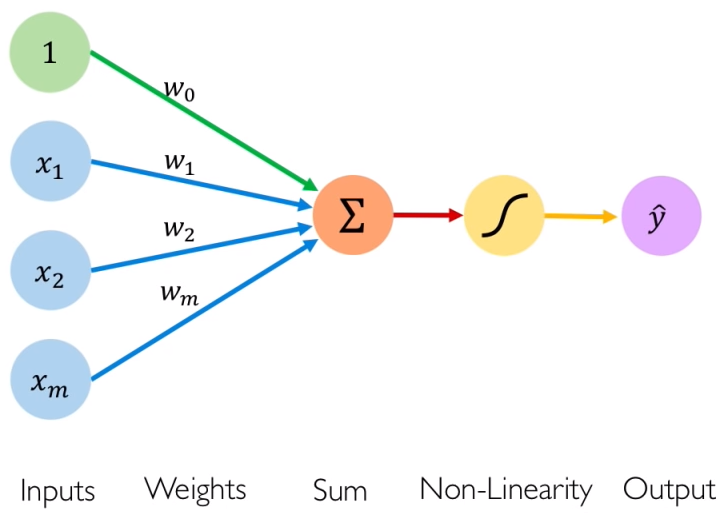
\includegraphics[width=0.5\textwidth,height=6cm,keepaspectratio=true]{content/images/PerzeptronVisualisierung.png}
    \caption{Grafische Visualisierung eines Perzeptrons als Grundbaustein von \acrshortpl{nn} \cite{6S191Intro}}
    \label{fig:PerzeptronVisualisierung}
\end{figure}

Ein Perzeptron hat eine beliebige Anzahl von Eingängen (engl. \emph{inputs}).
Die Eingänge $x_1 \dots x_n$ werden mit den Gewichtungen (engl. \emph{weights}) $w_1 \dots w_m$ multipliziert und die Ergebnisse aufsummiert.
Unabhängig von den Eingängen wird dann noch ein Bias $w_0$ dazu addiert.
Zuletzt wird eine nicht-lineare Aktivierungsfunktion $g$ auf das Ergebnis angewendet.
Bekannte Aktivierungsfunktionen sind z.\,B. \emph{Sigmoid} oder \emph{\acrfullr{relu}}, wobei in der Praxis meistens \emph{\acrshort{relu}} verwendet wird \cite{ActivFuncSharma,ActivFuncNwankpa}.
Die gesamte Berechnung des Ausgangs $\hat{y}$ ist in der aus \cite{6S191Intro} übernommenen \autoref{eq:PerceptronEquation} zu sehen.

\begin{equation}
    \hat{y} = g\left(w_0 + \sum_{i=1}^{m} x_i w_i \right)  
\label{eq:PerceptronEquation}
\end{equation}

Ein neuronales Netz entsteht nun, wenn mehrere dieser Perzeptronen kombiniert werden.
Die einfachste Möglichkeit ist ein sogenanntes Fully-connected Feedforward-Netz.
Hierbei werden mehrere Schichten aus parallel angeordneten Perzeptronen gebildet.
Dies ist schematisch in \autoref{fig:FCNN} dargestellt.

\begin{figure}[h]
    \centering
    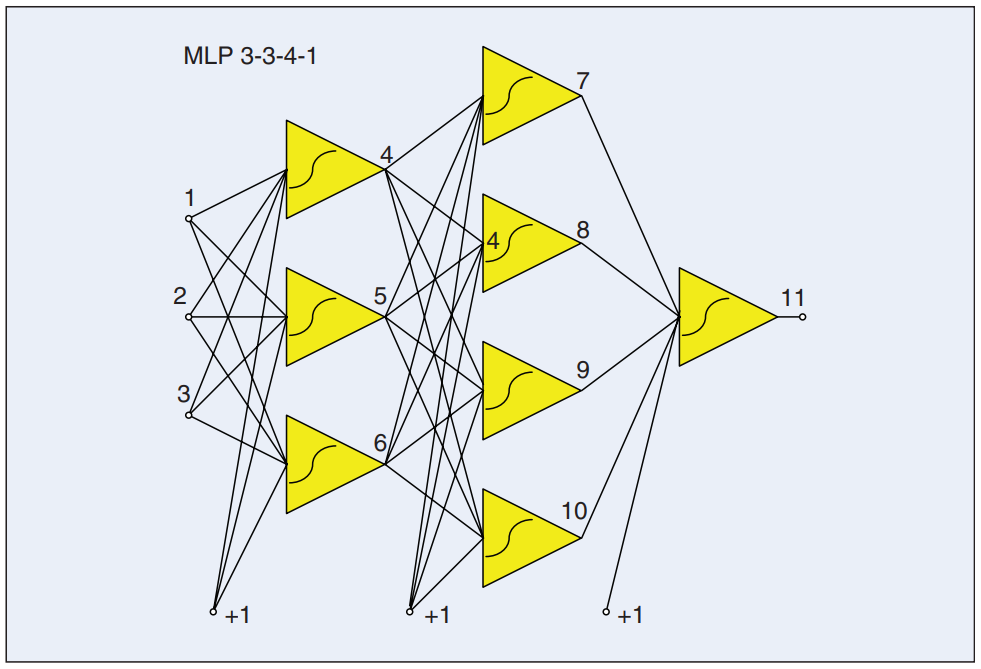
\includegraphics[width=1\textwidth,height=8cm,keepaspectratio=true]{content/images/FCNN.png}
    \caption{Architektur eines Fully-connected \acrshort{nn} \cite[FIGURE 1]{NNArchitectures}}
    \label{fig:FCNN}
\end{figure}

Wie in der Abbildung zu sehen ist, ist der Ausgang eines jeden Perzeptrons mit jedem Perzeptron der nächsten Schicht verbunden.
Der häufig verwendete Begriff \emph{Deep Learning} bezieht sich nach \cite[S. 27]{DeepLearningPythonKeras} auf die Vorgehensweise, Perzeptronen in mehreren Schichten anzuordnen.
Der Hintergedanke dabei ist nach \cite{6S191Intro}, dass durch die Schichten eine Merkmalshierarchie aufgebaut werden soll.
Bei der Erkennung von handgeschriebenen Ziffern könnte die erste Schicht beispielsweise Ecken und Kanten erkennen.
Die zweite Schicht würde aus Ecken und Kanten zusammengesetzte Kreise und Linien erkennen.
Schließlich könnte die dritte Schicht komplette Ziffern erkennen, die wiederum aus Linien und Kreisen zusammengesetzt sind.

Bisher wurde nur das eigentliche \acrshort{nn} erklärt.
Um ein \acrshort{nn} zu trainieren, sind jedoch noch einige andere Komponenten notwendig.
Das Zusammenspiel dieser Komponenten ist in \autoref{fig:DLKomponenten} dargestellt.
\begin{figure}[h]
    \centering
    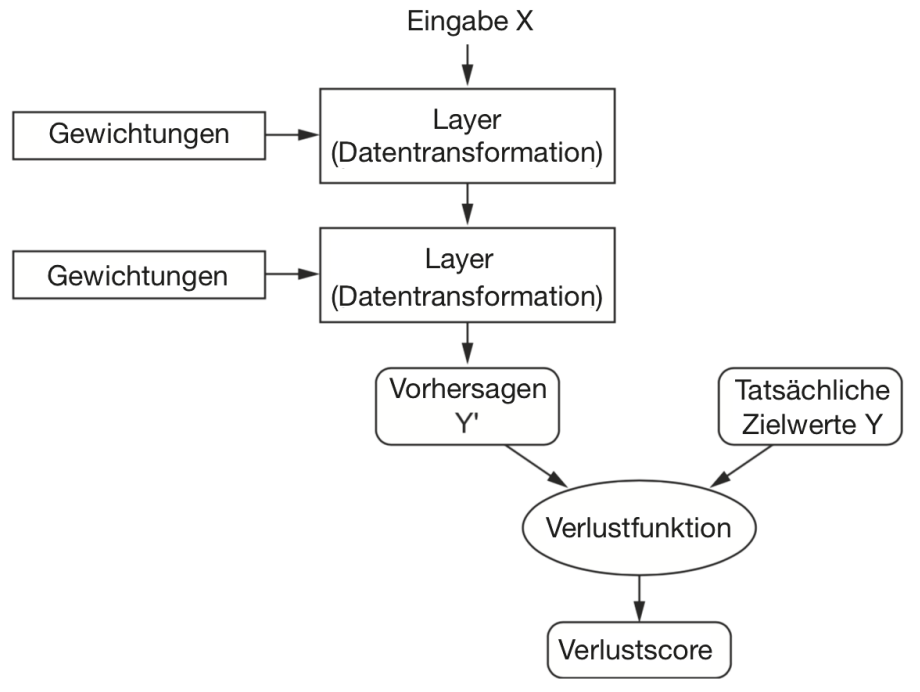
\includegraphics[width=1\textwidth,height=8cm,keepaspectratio=true]{content/images/DeepLearningKomponenten.png}
    \caption{Komponenten eines Deep Learning Systems \cite[Abb. 1.9]{DeepLearningPythonKeras}}
    \label{fig:DLKomponenten}
\end{figure}
Wie in der Abbildung erkennbar ist, wird eine Verlustfunktion benötigt.
Diese erhält nach \cite[S. 30]{DeepLearningPythonKeras} als Eingabe die Vorhersagen $Y'$ des \acrshort{nn}s sowie die tatsächlichen Werte $Y$.
Die Verlustfunktion berechnet anhand dieser Eingaben einen Verlustscore (engl. \emph{loss}), der ein Maß dafür ist, wie stark die Vorhersagen von den tatsächlichen Werten abweichen.
Die Ausgabe der Verlustfunktion ist umso größer, je stärker diese Abweichung ist.
Es gibt viele verschiedene Verlustfunktionen, die für unterschiedliche Aufgabenstellungen geeignet sind.
Häufig verwendet werden nach \cite[S. 155]{DeepLearningPythonKeras} z.\,B. der mittlere quadratische Fehler (engl. \acrfull{mse}) oder die binäre Kreuzentropie (engl. \emph{binary crossentropy}).

Als letzte wichtige Komponente wird noch ein Optimierer benötigt.
Dieser erhält als Eingabe den Verlustscore und passt anhand dessen die Gewichtungen des \acrshort{nn}s so an, dass der Verlustscore minimiert wird.
Hierfür wird laut \cite[S. 30]{DeepLearningPythonKeras} ein Algorithmus namens \emph{Backpropagation} verwendet.
Von diesem allgemeinen Algorithmus gibt es viele verschiedene Implementierungen, die sogenannten Optimierer.
In der vorliegenden Arbeit wird der in \cite{AdamPaper} vorgestellte \emph{Adam}-Optimierer verwendet.
Die Vorteile dieses Optimierers sind, den Autoren zufolge, die einfache Implementierung sowie die Speicher- und Recheneffizienz.

Zusammengefasst ist Deep Learning nichts anderes als eine Funktionsminimierung.
Die bedeutende Errungenschaft dabei ist, dass die große Menge an Gewichtungen (bei größeren \acrshort{nn}s mehrere Millionen) effizient angepasst werden können, sodass der Verlustscore minimiert wird.

